\documentclass{beamer}

%\usetheme[
%    block=fill,
%    background=light,
%    titleformat=smallcaps,
%    numbering=none
%]{default}

\usepackage{tabularx}
\usepackage{wasysym}
\usepackage{amsmath}
\usepackage{amssymb}
\usepackage{mathtools}
\usepackage{proof}
\usepackage{pifont}
\usepackage{algpseudocode}
\usepackage{algorithmicx}
\usepackage{tikz}
\usetikzlibrary{decorations.pathmorphing}
\usetikzlibrary{arrows.meta}
\usetikzlibrary{calc}
\usetikzlibrary{matrix}
\usetikzlibrary{positioning}
\usepackage{soul}
\usepackage{qtree}


\title{Types, Networks \& Stuff}
\institute{LoLa 2019}
\author{Kokos}
\date{7 January 2020}

\algnewcommand\algorithmicforeach{\textbf{for each}}
\algdef{S}[FOR]{ForEach}[1]{\algorithmicforeach\ #1\ \algorithmicdo}

\begin{document}

\maketitle

\begin{frame}{Overview}
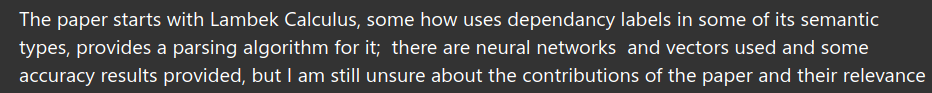
\includegraphics[keepaspectratio,width=\textwidth]{intro.png}\vfill

\pause
\begin{itemize}
	\item[$\lambda$] Abstract Syntax with NLP
	\item[$\lambda$] Extracting \& Learning Type Assignments
	\item[$\lambda$] Navigating proofs with neural nets
	\item[$\lambda$] Lexicalized syntax in language modeling
\end{itemize}

\end{frame}

\begin{frame}{This Timeline}
	\begin{tikzpicture}
		\node (syntax) at (0,0) {\scriptsize Syntactic Derivations};	
		\node (nl) at (0,0.7) {\scriptsize (N)L};
		\node (der) at (4,0) {\scriptsize Derivational Semantics};
		\node (mill) at (4,0.7) {\scriptsize LP};
		\node (sem) at (8,0) {\scriptsize Lexical Semantics};
		\node (il) at (8, 0.7) {\scriptsize IL};

		\draw (syntax) edge[->] node[midway, above] {\footnotesize $h_{der}$} (der);
		\draw (der) edge[->] node[midway, above] {\footnotesize $h_{lex}$} (sem);
	\end{tikzpicture}	
\end{frame}

\begin{frame}{Alternative Timeline}
	\begin{tikzpicture}
		\visible<2->{
			\node (syntax) at (0,0) {\scriptsize \color{gray}{Syntactic Derivations}};
			\node (nl) at (0, 0.5) {\scriptsize \color{gray}{?}};}			
%		\node (abstract) at (2, 2) {\scriptsize wtf};		
		\node (der) at (4,1.5) {\scriptsize \color{red}{Abstract Syntax}};
		\node (nlp) at (4, 2.2) {\scriptsize \color{red}{NLP}};
		\node (sem) at (8,0) {\scriptsize Lexical Semantics};
		\node (il) at (8, 0.7) {\scriptsize IL};
		
		\visible<2->{\draw (der) edge[->, gray] node[midway, above] {\footnotesize \color{gray}{?}} (syntax);}
		\draw (der) edge[->] node[midway, above] {\footnotesize $h_{lex}$} (sem);		
	\end{tikzpicture}
\end{frame}

\begin{frame}{NLP}

	\begin{block}{Grammar}
		IILL + Structural Control Modalities
	\end{block}
	\vfill	
	
	\[
		\mathcal{T} := A \ | \ \diamond^d{T}_1 \to T_2 \
	\]
	\vfill 
	
	\begin{align*}
		A \in \mathcal{A} &{\quad::\quad} 
			\text{Atoms denoting complete phrases \scriptsize {(NP, S, \dots)}}\\
		d \in \mathcal{D} &{\quad::\quad}  
			\text{Grammatical relations \scriptsize{(subject, object, \dots)}} \\
		\diamond^dT &{\quad::\quad} 
			\text{Type demarkated by \textit{dependency domain} d}\\
		T_1 \to T_2 &{\quad::\quad} 
			\text{Linear functor from $T_1$ to $T_2$}
	\end{align*}
\end{frame}


\begin{frame}{	
\includegraphics[keepaspectratio,width=\textwidth]{but_why.png}	}
	
	\textbf{Why?}
	\begin{itemize}
		\item Easier to extract from corpora
		\item Drastic reduction in lexical ambiguity
		\item More informative for semantics
		\item Built-in Interpretability
		\item Diamonds can regulate parsing (?)
	\end{itemize}\vfill	
	
	\pause
	\textbf{How?}
	\small
		\begin{equation*}
			\infer[\to  E]{\Gamma,\Delta\vdash (M\ N): {B}}{\Gamma\vdash M: A \to {B} & \Delta\vdash N: {A}}
		\end{equation*}
		\begin{equation*}
		    \infer[\to I]{\Gamma \vdash \lambda x.M: {A}\to {B}}{\Gamma, x: {A} \vdash M: {B}}
		\end{equation*}
		\begin{equation*}
		    \infer[\diamond^d I]{\langle \Gamma \rangle^d \vdash \diamond^d {A}}{\Gamma \vdash {A}}
		\end{equation*}
		\begin{equation*}
			\infer[\diamond^d E]{\Gamma,\Delta \vdash {B}}{\Delta \vdash \diamond^d {A}
			&
			\Gamma,\langle {A} \rangle^d \vdash {B}}
		\end{equation*}	
\end{frame}

\begin{frame}{}
	\centering
	\alert{
		A dataset of types \& proofs
	}
\end{frame}

\begin{frame}{Extracting (1/3)}
\small

	\begin{block}{Algorithm}
		Graph flooding on syntactic parse graphs \\
		Init with maps:
		\begin{itemize}
			\item[-] from POS/Phrasal-tags to atoms
			\item[-] dependency labels to diamond operators
		\end{itemize}
		Two subroutines;
			each \textit{selects} untyped nodes and \textit{types} them
	\end{block}
	
	\pause	
	\vfill
	\begin{algorithmic}
	\Function{TypeDag: DAG $D$ $\to$ DAG}{}
		\State $D$ $\gets$ DetachNonLocal($D$)
		\While{$D$ is not fully typed}
			\State $D$ $\gets$ TypeStandaloneNodes($D$)
			\State $D$ $\gets$ TypeHeadsAndMods($D$)
		\EndWhile\\
		\Return AttachNonLocal($D$)
	\EndFunction
	\end{algorithmic}
\end{frame}

\begin{frame}{Extracting (2/3)}
\small

	\begin{itemize}
		\item[$\lambda$1] Stand-Alone Nodes
			\begin{itemize}
				\setlength{\itemindent}{.25in}
				\item[select] untyped nodes with
					\begin{itemize}
						\item[1] no incoming head/mod edge
						\item[2] no untyped daughters (except heads/mods)
					\end{itemize}
				\item[type] translate pos/tag to atom
			\end{itemize}\vfill
		\item[$\lambda$2] Heads and Mods
			\begin{itemize}
				\setlength{\itemindent}{.25in}
				\item[select] untyped nodes that
					\begin{itemize}
						\item[1] incoming head/mod edge
						\item[2] have a typed parent
						\item[3] have all sisters (except head/mods) typed
					\end{itemize}
				\item[type] endofunctor of parent if mod, else functor from vector of arguments\footnote{minus hypotheses} to parent type
			\end{itemize}
	\end{itemize}

\end{frame}


\begin{frame}{Extracting (3/3)}

	\begin{block}{Non-Local Dependencies}
	\begin{algorithmic}
	\Function{DetachNonLocal: DAG $D$ $\to$ Tree}{}
		\ForEach {$e$ $\in$ $\textsc{Filter(Reentrant}, D.edges)$}
			\State $c$ $\gets$ copy$(e.target)$
			\State $D.nodes$ $\gets$ $D.nodes \cup \{c\}$
			\State $D.edges$ $\gets$ $D.edges - \{e\}$
			\State $D.edges$ $\gets$ $D.edges \cup \{(e.source, e.label, c)\}$
		\EndFor\\
		\Return $D$
	\EndFunction
	\end{algorithmic}
	\end{block}	
\end{frame}

\begin{frame}{}
	\centering
		\alert{Mommy, where do types come from?}

\end{frame}

\begin{frame}{Lexical Type Ambiguity}

	\begin{block}{Word/Type histogram}
	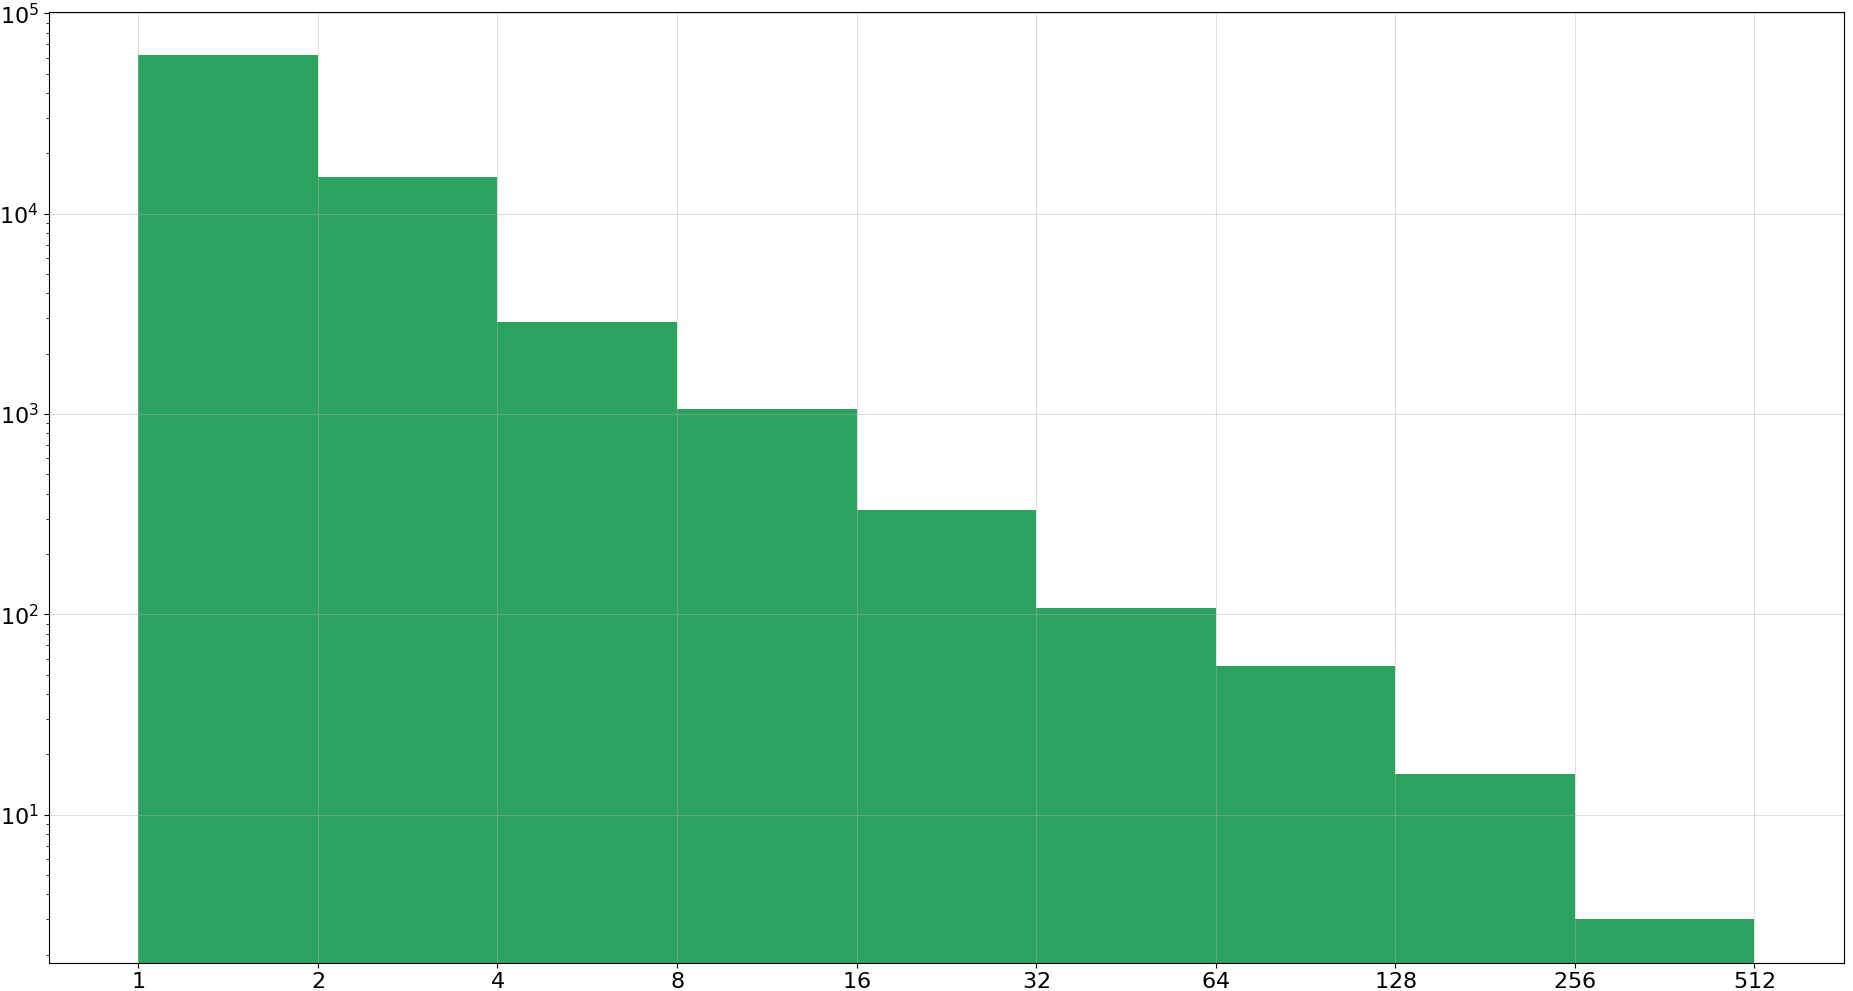
\includegraphics[keepaspectratio,width=\textwidth]{oracle.png}
	\end{block}
\end{frame}

\begin{frame}{Supertagging (\alt<3->{2}{1}/3)}
	\small	
	
	\begin{block}{General idea}
		\[
			p(t_1, t_2, \dots t_n | w_1, w_2, \dots w_n, \theta)
		\]
	\end{block}\vfill
	
	\begin{block}{\alt<3->{\st{Markov Assumption}}{Markov Assumption}}
		\alt<3->{
		\[
			\approx \prod_{i=1}^n p(t_i | t_1, \dots t_{i-1}, w1, \dots, w_n, \theta)
		\]
		}{
		\[
			\approx \prod_{i=1}^n p(t_i | w_1, w_2, \dots w_n, \theta)
		\]
		}
	\end{block}\vfill

	\begin{itemize}
		\item[\smiley] Seq2Seq \alt<3->{\alert{Transduction}}{Classification}
		\item[\alt<3->{\smiley}{\frownie}] \alt<3->{\alert{Many Answers}}{Single Answer}
		\item[\frownie] Sample Sparsity
		\item[\frownie] Closed Domain Assumption 
	\end{itemize}
\end{frame}

\begin{frame}{Supertagging (3/3)}
	\small
	\begin{block}{A step further}
		The syntax of the type system forms a simple CFG
		\begin{align*}
			S & \implies A \  &\forall \ A \ \in \ \mathcal{A}\\
			S & \implies d \ S \ S \ &\forall \ d \ \in \ \mathcal{D}
		\end{align*}
	\end{block}
	
	\pause
	\begin{itemize}
		\item Supertagging as conditional CFG generation
		\item CFG terminals as decoding targets
			\[
			\approx \prod_{i=1}^{\alert{m}} p(\alert{\sigma_i} | \alert{\sigma_1}, \dots \alert{\sigma_{i-1}}, w1, \dots, w_n, \theta)
			\]
			\[
				\sigma \in \mathcal{A} \cup \mathcal{D} \cup \{ \textsc{\scriptsize <SEP>} \}
			\]
	\end{itemize}
	
	\pause
	\begin{itemize}
		\item[\smiley] \st{Sample Sparsity} Many (sub)type examples
		\item[\smiley] \st{Closed Domain Assumption} Inductive construction of any type
	\end{itemize}
	
\end{frame}

\begin{frame}{}
	\centering
	\alert{
		Structural Ambiguity
	}
\end{frame}

\begin{frame}{Navigating Proofs}	

	\begin{block}{Parse State}
		\begin{itemize}
			\item A logical judgement (premises \& conclusion)
			\item Word associations for (some) premise formulas
			\item A single element stack
		\end{itemize}
	\end{block}
	
	\pause
	\begin{block}{Framework}	
		Given a parse state:
		\begin{itemize}
			\item[1] Decide between introduction $\oplus$ elimination
			\item[2] Perform either
			\item[3] Update state(s) 
			\item[4] Repeat
		\end{itemize}		
	\end{block}
\end{frame}

\begin{frame}{Proof Ambiguity}

	\begin{block}{The Problem}
		\begin{itemize}
			\item Introduction steps are deterministic
			\item Eliminations are not
		\end{itemize}
	\end{block}\vfill
	
	\pause
	\begin{block}{Key Insight}
		Elimination branching $\sim$ binary sequence chunking\\
		Semantic content can help disambiguate structure\\
	\end{block}\vfill
	
\end{frame}

\begin{frame}{Vectorizing Types}	
	\small
	
	\begin{block}{Types are trees}
	\centering 
	\[
		\diamond^{body}(\diamond^{su} NP \to S) \to \diamond^{mod} NP \to NP
	\]
	\end{block}

	\centering
	{\scriptsize
	\begin{minipage}{0.5\textwidth}
		\Tree[.{$\to$}	[.{$\diamond \ body$} [.{$\to$} [.{$\diamond \ {su}$} NP ] S ] ] [.{$\to$} [.{$\diamond \ mod$} NP ] NP ] ] 
	\end{minipage}
	}\vfill
	
	\pause
	\centering
	\begin{itemize}
		\item Atoms as vectors in $\mathbb{R}^n$
		\item Dependencies as functions $\mathbb{R}^n \to \mathbb{R}^n \to \mathbb{R}^n$
	\end{itemize}
\end{frame}

\begin{frame}{Proof Traversal}

    {
    \scriptsize
    \begin{minipage}{0.3\textheight}
    	\infer[]{\text{ducks}, \text{have}, \text{many}, \text{predators} \vdash \text{S}}{
	    	\infer[Ax.]{\text{\color<2>{red} ducks} \vdash \text{NP}}{}
	    	&
	    	\hspace{-20pt}
    		\infer[\rightarrow E]{\text{have}, \text{many}, \text{predators} \vdash \text{NP} \to \text{S}}{
    			\infer[\rightarrow E]{\text{\color<4>{red}many}, \text{\color<4>{red}predators} \vdash \text{NP}}{
    				\infer[Ax.]{\text{\color<6>{red} predators} \vdash \text{NP}}{}
    				&
    				\infer[Ax.]{\text{many} \vdash \text{NP} \to \text{NP}}{}
    			}
    			&
    			\infer[Ax.]{\text{have} \vdash \text{NP} \to \text{NP} \to \text{S}}{}
    		}
    	} 
    \end{minipage}
    }\vfill
    
    \begin{minipage}{0.6\textheight}
    \begin{figure}
    \centering
    \begin{tikzpicture}
        \scriptsize
        
    	\node[rectangle, inner sep=0pt, minimum width=120pt, minimum height=20pt] (ducks) at (0, -1.5) {
    		\alt<3->{
    			\alt<5->{
    				\alt<7->{
    					\alt<9->{}
    						{}}
    				{many, {\color<6->{red}predators}}}
    			{have, {\color<4->{red}many, predators}}}
    		{{\color<2->{red}ducks}, have, many, predators}
			\alt<7->{}{$\vdash$}
			\alt<3->{
				\alt<5->{
					\alt<7->{}
					{NP}}
				{NP $\to$ S}}
			{S}
		};
    	

   	\node[draw=white, rectangle, minimum width=240pt, minimum height=20pt, ultra thick, fill=black] (bb) at (0, 0) {\color{white}{Sequence Processing Black Box}};
   	
    	\pause
    	\node[rectangle, inner sep=0pt, minimum width=120pt, minimum height=20pt] (ducks) at (0, -1.5) {};
    	\invisible<7->{\draw ($(ducks.north) + (0, 0)$) edge[->, ultra thick] node[above] {} ($(bb.south) + (0, 0)$);}
    	
		\node[rectangle, inner sep=0pt, minimum width=120pt, minimum height=20pt] (fst) at (-2.25, 1.25) {
		{\alt<3->{}{{\color{red} L}}}};
		
		\node[rectangle, inner sep=0pt, minimum width=120pt, minimum height=20pt] (snd) at (-1.25, 1.25) {
		{\alt<3->{
			\alt<4->{
				\alt<5->{
					\alt<6->{\invisible<7->{R}}{}}{R}}{}
%					\alt<6->{}{}}{R}}{}
		}{R}}};
		
		\node[rectangle, inner sep=0pt, minimum width=120pt, minimum height=20pt] (trd) at (-0.25, 1.25) {
		{\alt<3->{
			\alt<4->{
				\alt<5->{
%					\alt<6->{\invisible<7->{R}}{}}{\color{red} L}}{}
					\alt<6->{\invisible<7->{\color{red} L}}{}}{\color{red} L}}{}

		}{R}}};
		
		\node[rectangle, inner sep=0pt, minimum width=120pt, minimum height=20pt] (fth) at (0.75, 1.25) {
		{\alt<3->{
			\alt<4->{
				\alt<5->{
					\alt<6->{}{}}{\color{red} L}}{}
		}{R}}};
		
		\invisible<3->{
			\draw ($(bb) + (-2.25, 0.25)$) edge[->, thick, red] node[above] {} ($(fst.south)$);
			\draw ($(bb) + (-1.25, 0.25)$) edge[->, thick] node[above] {} ($(snd.south)$);
			\draw ($(bb) + (-0.25, 0.25)$) edge[->, thick] node[above] {} ($(trd.south)$);
			\draw ($(bb) + (0.75, 0.25)$) edge[->, thick] node[above] {} ($(fth.south)$);
		}
		
	\alt<4->{
	\invisible<5->{
			\draw ($(bb) + (-1.25, 0.25)$) edge[->, thick] node[above] {} ($(snd.south)$);
			\draw ($(bb) + (-0.25, 0.25)$) edge[->, thick, red] node[above] {} ($(trd.south)$);
			\draw ($(bb) + (0.75, 0.25)$) edge[->, thick, red] node[above] {} ($(fth.south)$);
		}
	}{}
	
	\alt<6->{
	\invisible<7->{
			\draw ($(bb) + (-1.25, 0.25)$) edge[->, thick] node[above] {} ($(snd.south)$);
			\draw ($(bb) + (-0.25, 0.25)$) edge[->, thick, red] node[above] {} ($(trd.south)$);
		}
	}{}
    \end{tikzpicture}
    \end{figure}
    \end{minipage} 
    \vfill 
   
	\only<8>{
	\[
	\begin{rcases*}
		\text{Training sample} \ &: \ \text{Elimination branching} \\
		\text{Sentence} \ 	&: \ \text{N \textit{independent} samples} \\
	\end{rcases*}  \text{\alert{Training Parallelism}}
	\]
    }
\end{frame}

\begin{frame}{}
	\centering
	\alert{
		Parsing in $\mathcal{O}$(1)
	}\footnote{
	\scriptsize Sensationalist}
\end{frame}


\begin{frame}{Parsing as Latent Permutation}
	\[
		\alt<2->{\alt<3->{np_1^+}{np_1}}{np}, 
		\alt<2->{\alt<3->{np_2^-}{np_2}}{np} 
		\to 
		\alt<2->{\alt<3->{np_3^-}{np_3}}{np} 
		\to 
		\alt<2->{\alt<3->{s_1^+}{s_1}}{s}, 
		\alt<2->{\alt<3->{np_4^-}{np_4}}{np} 
		\to \alt<2->{\alt<3->{np_5^+}{np_5}}{np}, 
		\alt<2->{\alt<3->{np_6^+}{np_6}}{np} 
		\vdash 
		\alt<2->{\alt<3->{s_2^-}{s_2}}{s}
	\]\vfill

	\pause
	\pause
	\pause
	
	\[
		P = [np_1, s_1, np_5, np_6] \quad 		N = [np_2, np_3, np_4, s_2]
	\]\vfill

	\pause	
	
	\centering
	\alt<6->{$\mathcal{R} \in \mathbb{B}^{4 \times 4}$ =}{} \begin{tabular}{c|cccc}
		& $np_2$ & $np_3$ & $np_4$ & $s_2$\\
		\hline
		$np_1$ & \visible<6-> 0 & \alt<6->{1}{X} & \visible<6-> 0 & \visible<6-> 0 \\
		$s_1$ &  \visible<6-> 0 &  \visible<6-> 0 &  \visible<6-> 0 & \alt<6->{1}{X} \\
		$np_5$ & \alt<6->{1}{X} & \visible<6-> 0 & \visible<6-> 0 &  \visible<6-> 0\\
		$np_6$ & \visible<6-> 0 & \visible<6-> 0 & \alt<6->{1}{X} &  \visible<6-> 0\\
	\end{tabular} 
	
	\pause
	\[
		\text{match}(N) = P\mathcal{R}^T
	\]
	
	\pause
	\begin{itemize}
		\item $\mathcal{R}$ is \textit{discrete}
		\pause
		\item .. but its continuous relaxations can be approximated (Sinkhorn-Knopp)
	\end{itemize}	
\end{frame}


\begin{frame}{References}
	\small 
	
	\begin{block}{Grammar \& Extraction}
		\begin{itemize}
			\item \AE THEL: Automatically Extracted Type-Logical Derivations for Dutch \href{https://arxiv.org/abs/1912.12635}{\color{blue}{link}}
		\end{itemize}
		
	\end{block}
	
	\begin{block}{Supertagging \& Parsing}
		\begin{itemize}
			\item Constructive Type-Logical Supertagging with Self-Attention Networks \href{https://arxiv.org/abs/1905.13418}{\color{blue}link}
			\item Deductive Parsing with an Unbounded Type Lexicon \href{https://hal-lirmm.ccsd.cnrs.fr/lirmm-02313572/document}{\color{blue}link}
		\end{itemize}
	\end{block}
	
	\begin{block}{Permutations}
		\begin{itemize}
		\item Sinkhorn-Knopp Algorithm \href{http://yaroslavvb.com/papers/sinkhorn-concerning.pdf}{\color{blue}link}
		\item Learning Latent Permutations with Gumbel-Sinkhorn Networks \href{https://arxiv.org/abs/1802.08665}{\color{blue}link}
		\end{itemize}
	\end{block}
\end{frame}

\end{document}